\documentclass[]{book}
\usepackage{lmodern}
\usepackage{amssymb,amsmath}
\usepackage{ifxetex,ifluatex}
\usepackage{fixltx2e} % provides \textsubscript
\ifnum 0\ifxetex 1\fi\ifluatex 1\fi=0 % if pdftex
  \usepackage[T1]{fontenc}
  \usepackage[utf8]{inputenc}
\else % if luatex or xelatex
  \ifxetex
    \usepackage{mathspec}
  \else
    \usepackage{fontspec}
  \fi
  \defaultfontfeatures{Ligatures=TeX,Scale=MatchLowercase}
\fi
% use upquote if available, for straight quotes in verbatim environments
\IfFileExists{upquote.sty}{\usepackage{upquote}}{}
% use microtype if available
\IfFileExists{microtype.sty}{%
\usepackage{microtype}
\UseMicrotypeSet[protrusion]{basicmath} % disable protrusion for tt fonts
}{}
\usepackage{hyperref}
\hypersetup{unicode=true,
            pdftitle={An Introduction to Data wrangling with R},
            pdfauthor={Juqiang Chen},
            pdfborder={0 0 0},
            breaklinks=true}
\urlstyle{same}  % don't use monospace font for urls
\usepackage{natbib}
\bibliographystyle{apalike}
\usepackage{color}
\usepackage{fancyvrb}
\newcommand{\VerbBar}{|}
\newcommand{\VERB}{\Verb[commandchars=\\\{\}]}
\DefineVerbatimEnvironment{Highlighting}{Verbatim}{commandchars=\\\{\}}
% Add ',fontsize=\small' for more characters per line
\usepackage{framed}
\definecolor{shadecolor}{RGB}{248,248,248}
\newenvironment{Shaded}{\begin{snugshade}}{\end{snugshade}}
\newcommand{\KeywordTok}[1]{\textcolor[rgb]{0.13,0.29,0.53}{\textbf{#1}}}
\newcommand{\DataTypeTok}[1]{\textcolor[rgb]{0.13,0.29,0.53}{#1}}
\newcommand{\DecValTok}[1]{\textcolor[rgb]{0.00,0.00,0.81}{#1}}
\newcommand{\BaseNTok}[1]{\textcolor[rgb]{0.00,0.00,0.81}{#1}}
\newcommand{\FloatTok}[1]{\textcolor[rgb]{0.00,0.00,0.81}{#1}}
\newcommand{\ConstantTok}[1]{\textcolor[rgb]{0.00,0.00,0.00}{#1}}
\newcommand{\CharTok}[1]{\textcolor[rgb]{0.31,0.60,0.02}{#1}}
\newcommand{\SpecialCharTok}[1]{\textcolor[rgb]{0.00,0.00,0.00}{#1}}
\newcommand{\StringTok}[1]{\textcolor[rgb]{0.31,0.60,0.02}{#1}}
\newcommand{\VerbatimStringTok}[1]{\textcolor[rgb]{0.31,0.60,0.02}{#1}}
\newcommand{\SpecialStringTok}[1]{\textcolor[rgb]{0.31,0.60,0.02}{#1}}
\newcommand{\ImportTok}[1]{#1}
\newcommand{\CommentTok}[1]{\textcolor[rgb]{0.56,0.35,0.01}{\textit{#1}}}
\newcommand{\DocumentationTok}[1]{\textcolor[rgb]{0.56,0.35,0.01}{\textbf{\textit{#1}}}}
\newcommand{\AnnotationTok}[1]{\textcolor[rgb]{0.56,0.35,0.01}{\textbf{\textit{#1}}}}
\newcommand{\CommentVarTok}[1]{\textcolor[rgb]{0.56,0.35,0.01}{\textbf{\textit{#1}}}}
\newcommand{\OtherTok}[1]{\textcolor[rgb]{0.56,0.35,0.01}{#1}}
\newcommand{\FunctionTok}[1]{\textcolor[rgb]{0.00,0.00,0.00}{#1}}
\newcommand{\VariableTok}[1]{\textcolor[rgb]{0.00,0.00,0.00}{#1}}
\newcommand{\ControlFlowTok}[1]{\textcolor[rgb]{0.13,0.29,0.53}{\textbf{#1}}}
\newcommand{\OperatorTok}[1]{\textcolor[rgb]{0.81,0.36,0.00}{\textbf{#1}}}
\newcommand{\BuiltInTok}[1]{#1}
\newcommand{\ExtensionTok}[1]{#1}
\newcommand{\PreprocessorTok}[1]{\textcolor[rgb]{0.56,0.35,0.01}{\textit{#1}}}
\newcommand{\AttributeTok}[1]{\textcolor[rgb]{0.77,0.63,0.00}{#1}}
\newcommand{\RegionMarkerTok}[1]{#1}
\newcommand{\InformationTok}[1]{\textcolor[rgb]{0.56,0.35,0.01}{\textbf{\textit{#1}}}}
\newcommand{\WarningTok}[1]{\textcolor[rgb]{0.56,0.35,0.01}{\textbf{\textit{#1}}}}
\newcommand{\AlertTok}[1]{\textcolor[rgb]{0.94,0.16,0.16}{#1}}
\newcommand{\ErrorTok}[1]{\textcolor[rgb]{0.64,0.00,0.00}{\textbf{#1}}}
\newcommand{\NormalTok}[1]{#1}
\usepackage{longtable,booktabs}
\usepackage{graphicx,grffile}
\makeatletter
\def\maxwidth{\ifdim\Gin@nat@width>\linewidth\linewidth\else\Gin@nat@width\fi}
\def\maxheight{\ifdim\Gin@nat@height>\textheight\textheight\else\Gin@nat@height\fi}
\makeatother
% Scale images if necessary, so that they will not overflow the page
% margins by default, and it is still possible to overwrite the defaults
% using explicit options in \includegraphics[width, height, ...]{}
\setkeys{Gin}{width=\maxwidth,height=\maxheight,keepaspectratio}
\IfFileExists{parskip.sty}{%
\usepackage{parskip}
}{% else
\setlength{\parindent}{0pt}
\setlength{\parskip}{6pt plus 2pt minus 1pt}
}
\setlength{\emergencystretch}{3em}  % prevent overfull lines
\providecommand{\tightlist}{%
  \setlength{\itemsep}{0pt}\setlength{\parskip}{0pt}}
\setcounter{secnumdepth}{5}
% Redefines (sub)paragraphs to behave more like sections
\ifx\paragraph\undefined\else
\let\oldparagraph\paragraph
\renewcommand{\paragraph}[1]{\oldparagraph{#1}\mbox{}}
\fi
\ifx\subparagraph\undefined\else
\let\oldsubparagraph\subparagraph
\renewcommand{\subparagraph}[1]{\oldsubparagraph{#1}\mbox{}}
\fi

%%% Use protect on footnotes to avoid problems with footnotes in titles
\let\rmarkdownfootnote\footnote%
\def\footnote{\protect\rmarkdownfootnote}

%%% Change title format to be more compact
\usepackage{titling}

% Create subtitle command for use in maketitle
\providecommand{\subtitle}[1]{
  \posttitle{
    \begin{center}\large#1\end{center}
    }
}

\setlength{\droptitle}{-2em}

  \title{An Introduction to Data wrangling with R}
    \pretitle{\vspace{\droptitle}\centering\huge}
  \posttitle{\par}
    \author{Juqiang Chen}
    \preauthor{\centering\large\emph}
  \postauthor{\par}
      \predate{\centering\large\emph}
  \postdate{\par}
    \date{2019-09-14}

\usepackage{booktabs}
\usepackage{amsthm}
\makeatletter
\def\thm@space@setup{%
  \thm@preskip=8pt plus 2pt minus 4pt
  \thm@postskip=\thm@preskip
}
\makeatother

\begin{document}
\maketitle

{
\setcounter{tocdepth}{1}
\tableofcontents
}
\chapter{Prerequisites}\label{prerequisites}

This document is to accompany \textbf{An introduction to data wrangling
with R} tutorial for DH Downunder 2019 at the University of Newcastle,
Australia, from 9-13 December.

I am a speech scientist working on cross-language lexical tone
perception and production. I have rich experience dealing with
experimental data and I am keen to help others with data wrangling, data
visualization and statistical modelling problems. I aspire to promote a
streamlined workflow with R packages to improve data analysis efficiency
in quantitative analysis in the field of social science and linguistics.

If you have any questions about the tutorial, please e-mail me at:
\href{mailto:j.chen2@westernsydney.edu.au}{\nolinkurl{j.chen2@westernsydney.edu.au}}

Good data are somewhat alike but messy data are messy in different ways.
This workshop aims to walk the audience through a streamlined workflow
of data wrangling (importing data, cleaning data, transforming data)
using popular R packages, such as dplyr and tidyr. It involves an
introduction to basic concepts in data analysis, such as variables
vs.~observations, categorical vs.~continuous variables, long vs.~wide
data. In addition, participants will learn how to (batch) import
datasets, select and rename rows and columns, deal with missing data,
generate new columns by computing the existing ones, and combine data
frames. The pipe operator will be introduced to improve the efficiency
and clarity of coding. Participants will also learn to write their own
functions for data wrangling. Exercises and challenges involve real life
research problems. Preliminary experience with R will be helpful, though
not required. Participants are required to download and install R and R
studio before the workshop. Datasets for the workshop are available
online before the workshop. Participants are welcomed to bring their own
data and apply what they learn on the spot.

Before we start our journey of data wrangling with R, you will need to
install R on your laptop. R is multi-platform, which means you can
install R on your PC or MAC.

\section{Installing R and R studio}\label{installing-r-and-r-studio}

Use this link {[}\url{https://cloud.r-project.org/}{]} to download R and
select the proper version for your laptop.

\begin{Shaded}
\begin{Highlighting}[]
\NormalTok{knitr}\OperatorTok{::}\KeywordTok{include_graphics}\NormalTok{(}\StringTok{"img/installr.jpg"}\NormalTok{)}
\end{Highlighting}
\end{Shaded}

\begin{figure}

{\centering 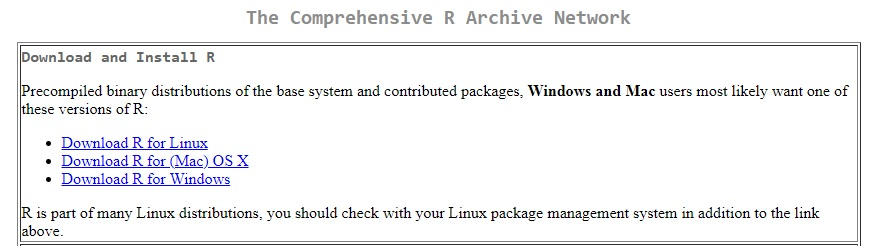
\includegraphics[width=1\linewidth]{img/installr} 

}

\caption{Download R}\label{fig:nice-fig}
\end{figure}

\section{Installing libraries in R}\label{installing-libraries-in-r}

RStudio is an integrated development environment, or IDE, for R
programming. Download and install it from
{[}\url{http://www.rstudio.com/download}.{]}

The \textbf{free version} is poweful enough.

\section{Install packages and library
packages}\label{install-packages-and-library-packages}

\begin{itemize}
\item
  install.packages(``package\_name'')
\item
  library(package\_name)
\end{itemize}

\section{Programme}\label{programme}

\textbf{Session 1} chapter 1 \& 2

\textbf{Session 2} chapter 3, 4 \& 5

\textbf{Session 3} chapter 3, 4 \& 5

\chapter{Basic data structures in R}\label{intro}

Before we get our hands dirty in doing actual data analysis, it is
desirable to first think about what types of variables and data
structures we are dealing with.

Before we talk about data structures in R, let's first think about how
data can be categorized.

\section{Nominal, ordinal, interval/ratio
variables}\label{nominal-ordinal-intervalratio-variables}

\begin{itemize}
\item
  \textbf{Nominal variables} are the data whose levels are labels or
  descriptions, which cannot be ordered. (e.g.~sex, school, or
  nationality). They are categorical in nature.
\item
  \textbf{Ordinal variables} can be ordered, or ranked in logical order,
  but the interval between levels of the variables are unknown.
\end{itemize}

\begin{quote}
For example, when doing a survey, participants will be asked to rate.
The subjective measurements of this kind are often ordinal variables.
E.g. a Likert ranking scale; level of education (``\textless{} high
school'', ``high school'', ``associate's degree'').
\end{quote}

We can assign numbers to levels of an ordinal variable, and can order
them, but we should bear in mind that these variable are not numeric.
For example, ``strongly agree'' and ``neutral'' cannot average out to an
``agree.'', even though you can assign 5 to ``strong agree'' and 3 to
``neutral''.

\begin{itemize}
\tightlist
\item
  \textbf{Interval/ratio variables} are measured or counted values: age,
  height, weight or number of students. The interval between numbers is
  equal: the interval between 1 kg and 2 kg is the same as between 3 kg
  and 4 kg. Interval/ratio variables can be \emph{discrete values}, such
  as population (1332) or counts of items, or they can be
  \emph{continuous variables} values that can take on any value within
  an interval, and can be expressed as decimals (1.009 kg).
\end{itemize}

The variable type will determine (1) statistical analysis; (2) the way
we summarize data with statistics and plots. We will be elaborating on
this in the \emph{Explorative Data Analysis course}.

Variables can be stored in R in different data types.

\begin{itemize}
\item
  Normial and ordinal variables can be stored as \emph{character} or
  \emph{factors} (with levels).
\item
  Interval data are stored as numbers either as \emph{integer} or
  \emph{numeric} (real or decimal).
\end{itemize}

If you have only one variable, you can store it in a vector. However,
more often than not, you have a bunch of variables that should be stored
or imported as a matrix or data frame.

\section{1D data structure: vectors}\label{d-data-structure-vectors}

A vector is a sequence of data elements of the same basic type: integer,
double, logical or character. All elements of a vector must be the same
type.

\subsection{Creating vectors}\label{creating-vectors}

\begin{Shaded}
\begin{Highlighting}[]
\NormalTok{a =}\StringTok{ }\DecValTok{8}\OperatorTok{:}\DecValTok{17}

\NormalTok{b <-}\StringTok{ }\KeywordTok{c}\NormalTok{(}\DecValTok{9}\NormalTok{, }\DecValTok{10}\NormalTok{, }\DecValTok{100}\NormalTok{, }\DecValTok{38}\NormalTok{)}

\NormalTok{c =}\StringTok{ }\KeywordTok{c}\NormalTok{ (}\OtherTok{TRUE}\NormalTok{, }\OtherTok{FALSE}\NormalTok{, }\OtherTok{TRUE}\NormalTok{, }\OtherTok{FALSE}\NormalTok{)}

\NormalTok{c =}\StringTok{ }\KeywordTok{c}\NormalTok{ (T, F, T, F)}

\NormalTok{d =}\StringTok{ }\KeywordTok{c}\NormalTok{ (}\StringTok{"TRUE"}\NormalTok{, }\StringTok{"FALSE"}\NormalTok{, }\StringTok{"FALSE"}\NormalTok{)}

\CommentTok{# You can change the type of a vector with as.vector function.}

\KeywordTok{as.vector}\NormalTok{(b, }\DataTypeTok{mode =} \StringTok{"character"}\NormalTok{)}
\end{Highlighting}
\end{Shaded}

\begin{verbatim}
## [1] "9"   "10"  "100" "38"
\end{verbatim}

\begin{Shaded}
\begin{Highlighting}[]
\CommentTok{# When you put elements of different types in one vector, R will automatically change the type of some elements to keep the whole vector homogenous.}

\NormalTok{e =}\StringTok{ }\KeywordTok{c}\NormalTok{(}\DecValTok{9}\NormalTok{,}\DecValTok{10}\NormalTok{, }\StringTok{"ab"}\NormalTok{, }\StringTok{"cd"}\NormalTok{)}

\NormalTok{f =}\StringTok{ }\KeywordTok{c}\NormalTok{(}\DecValTok{10}\NormalTok{, }\DecValTok{11}\NormalTok{, T, F)}
\end{Highlighting}
\end{Shaded}

c () is a function in R.

There are some other basic functions in R that you can play with to
generate vectors.

\begin{Shaded}
\begin{Highlighting}[]
\NormalTok{A =}\StringTok{ }\DecValTok{9}\OperatorTok{:}\DecValTok{20} \OperatorTok{+}\StringTok{ }\DecValTok{1}

\NormalTok{B =}\StringTok{ }\KeywordTok{seq}\NormalTok{ (}\DecValTok{1}\NormalTok{, }\DecValTok{10}\NormalTok{)}

\NormalTok{C =}\StringTok{ }\KeywordTok{seq}\NormalTok{ (}\DecValTok{1}\NormalTok{, }\DecValTok{20}\NormalTok{, }\DataTypeTok{by=} \DecValTok{2}\NormalTok{)}

\NormalTok{D =}\StringTok{ }\KeywordTok{rep}\NormalTok{ (}\DecValTok{5}\NormalTok{, }\DecValTok{4}\NormalTok{)}

\NormalTok{E =}\StringTok{ }\KeywordTok{rep}\NormalTok{ (}\KeywordTok{c}\NormalTok{(}\DecValTok{1}\NormalTok{,}\DecValTok{2}\NormalTok{,}\DecValTok{3}\NormalTok{), }\DecValTok{4}\NormalTok{)}

\NormalTok{G =}\StringTok{ }\KeywordTok{rep}\NormalTok{ (}\KeywordTok{c}\NormalTok{(}\DecValTok{1}\NormalTok{,}\DecValTok{2}\NormalTok{,}\DecValTok{3}\NormalTok{), }\DataTypeTok{each =} \DecValTok{4}\NormalTok{)}

\CommentTok{# Now that you have a vector, you can do some Maths.}

\KeywordTok{max}\NormalTok{(a)}
\end{Highlighting}
\end{Shaded}

\begin{verbatim}
## [1] 17
\end{verbatim}

\begin{Shaded}
\begin{Highlighting}[]
\KeywordTok{min}\NormalTok{(a)}
\end{Highlighting}
\end{Shaded}

\begin{verbatim}
## [1] 8
\end{verbatim}

\begin{Shaded}
\begin{Highlighting}[]
\KeywordTok{range}\NormalTok{(a)}
\end{Highlighting}
\end{Shaded}

\begin{verbatim}
## [1]  8 17
\end{verbatim}

\begin{Shaded}
\begin{Highlighting}[]
\KeywordTok{sum}\NormalTok{(a)}
\end{Highlighting}
\end{Shaded}

\begin{verbatim}
## [1] 125
\end{verbatim}

\begin{Shaded}
\begin{Highlighting}[]
\KeywordTok{mean}\NormalTok{(a)}
\end{Highlighting}
\end{Shaded}

\begin{verbatim}
## [1] 12.5
\end{verbatim}

\begin{Shaded}
\begin{Highlighting}[]
\KeywordTok{median}\NormalTok{(a)}
\end{Highlighting}
\end{Shaded}

\begin{verbatim}
## [1] 12.5
\end{verbatim}

\begin{Shaded}
\begin{Highlighting}[]
\KeywordTok{quantile}\NormalTok{(a)}
\end{Highlighting}
\end{Shaded}

\begin{verbatim}
##    0%   25%   50%   75%  100% 
##  8.00 10.25 12.50 14.75 17.00
\end{verbatim}

\begin{Shaded}
\begin{Highlighting}[]
\KeywordTok{sd}\NormalTok{(a)}
\end{Highlighting}
\end{Shaded}

\begin{verbatim}
## [1] 3.02765
\end{verbatim}

\begin{Shaded}
\begin{Highlighting}[]
\KeywordTok{round}\NormalTok{(}\KeywordTok{sd}\NormalTok{(a), }\DecValTok{2}\NormalTok{)}
\end{Highlighting}
\end{Shaded}

\begin{verbatim}
## [1] 3.03
\end{verbatim}

\subsection{creating list objects}\label{creating-list-objects}

We can put vectors of different types (e.g., number, logic or character)
and lengths in a list object.

\begin{Shaded}
\begin{Highlighting}[]
\NormalTok{list1 =}\StringTok{ }\KeywordTok{list}\NormalTok{(a, b, c, d, e, f)}

\NormalTok{list1}
\end{Highlighting}
\end{Shaded}

\begin{verbatim}
## [[1]]
##  [1]  8  9 10 11 12 13 14 15 16 17
## 
## [[2]]
## [1]   9  10 100  38
## 
## [[3]]
## [1]  TRUE FALSE  TRUE FALSE
## 
## [[4]]
## [1] "TRUE"  "FALSE" "FALSE"
## 
## [[5]]
## [1] "9"  "10" "ab" "cd"
## 
## [[6]]
## [1] 10 11  1  0
\end{verbatim}

\begin{Shaded}
\begin{Highlighting}[]
\CommentTok{# More often than not, we do not make list ourselves but have to deal with lists when we get outputs from stats models.}
\end{Highlighting}
\end{Shaded}

\section{2D data structures: matrice and data
frames}\label{d-data-structures-matrice-and-data-frames}

Most of us have had some experience with the Excel spreadsheet. Data in
a spreadsheet are arranged by rows and columns in a rectangular space.
This is a typical 2 dimensional data structure. In R, we can have two
ways of forming tabular data like a spreadsheet: the matrix and
dataframe.

\textbf{A matrix }is a collection of data elements arranged in a
two-dimensional rectangular layout in which all the elements must be of
the same type (e.g., numeric or character).

\textbf{Dataframe} is similar to matrix in shape but only differs in
that different types of data can co-exist in different columns. Thus, in
data analysis, we use dataframes more often than matrix.

\begin{Shaded}
\begin{Highlighting}[]
\CommentTok{# Let's generate a dataframe from scratch.}

\NormalTok{id =}\StringTok{ }\KeywordTok{seq}\NormalTok{(}\DecValTok{1}\NormalTok{, }\DecValTok{40}\NormalTok{)}

\NormalTok{gender =}\StringTok{ }\KeywordTok{rep}\NormalTok{(}\KeywordTok{c}\NormalTok{(}\StringTok{"male"}\NormalTok{, }\StringTok{"female"}\NormalTok{), }\DecValTok{5}\NormalTok{)}

\NormalTok{maths =}\StringTok{ }\KeywordTok{rnorm}\NormalTok{(}\DecValTok{40}\NormalTok{, }\DataTypeTok{mean =} \DecValTok{70}\NormalTok{, }\DataTypeTok{sd =} \DecValTok{5}\NormalTok{)}

\NormalTok{english =}\StringTok{ }\KeywordTok{rnorm}\NormalTok{(}\DecValTok{40}\NormalTok{, }\DataTypeTok{mean =} \DecValTok{80}\NormalTok{, }\DataTypeTok{sd =} \DecValTok{9}\NormalTok{)}

\NormalTok{music =}\StringTok{ }\KeywordTok{rnorm}\NormalTok{(}\DecValTok{40}\NormalTok{, }\DataTypeTok{mean =} \DecValTok{75}\NormalTok{, }\DataTypeTok{sd =} \DecValTok{10}\NormalTok{)}

\NormalTok{pe =}\StringTok{ }\KeywordTok{rnorm}\NormalTok{(}\DecValTok{40}\NormalTok{, }\DataTypeTok{mean =} \DecValTok{86}\NormalTok{, }\DataTypeTok{sd =} \DecValTok{12}\NormalTok{)}

\NormalTok{df1 =}\StringTok{ }\KeywordTok{data.frame}\NormalTok{ (id, gender, maths, english)}
\end{Highlighting}
\end{Shaded}

Now let's explore the data frame we just created.

\begin{Shaded}
\begin{Highlighting}[]
\KeywordTok{str}\NormalTok{(df1)}
\end{Highlighting}
\end{Shaded}

\begin{verbatim}
## 'data.frame':    40 obs. of  4 variables:
##  $ id     : int  1 2 3 4 5 6 7 8 9 10 ...
##  $ gender : Factor w/ 2 levels "female","male": 2 1 2 1 2 1 2 1 2 1 ...
##  $ maths  : num  72.8 62.8 76.6 65.8 67.7 ...
##  $ english: num  89.7 98.5 87.9 83.9 77.7 ...
\end{verbatim}

\begin{Shaded}
\begin{Highlighting}[]
\KeywordTok{summary}\NormalTok{(df1)}
\end{Highlighting}
\end{Shaded}

\begin{verbatim}
##        id           gender       maths          english      
##  Min.   : 1.00   female:20   Min.   :62.43   Min.   : 62.72  
##  1st Qu.:10.75   male  :20   1st Qu.:65.90   1st Qu.: 76.48  
##  Median :20.50               Median :70.63   Median : 81.48  
##  Mean   :20.50               Mean   :69.76   Mean   : 82.94  
##  3rd Qu.:30.25               3rd Qu.:72.70   3rd Qu.: 89.94  
##  Max.   :40.00               Max.   :77.53   Max.   :104.35
\end{verbatim}

\begin{Shaded}
\begin{Highlighting}[]
\KeywordTok{nrow}\NormalTok{(df1)}
\end{Highlighting}
\end{Shaded}

\begin{verbatim}
## [1] 40
\end{verbatim}

\begin{Shaded}
\begin{Highlighting}[]
\KeywordTok{ncol}\NormalTok{(df1)}
\end{Highlighting}
\end{Shaded}

\begin{verbatim}
## [1] 4
\end{verbatim}

\begin{Shaded}
\begin{Highlighting}[]
\KeywordTok{attributes}\NormalTok{(df1)}
\end{Highlighting}
\end{Shaded}

\begin{verbatim}
## $names
## [1] "id"      "gender"  "maths"   "english"
## 
## $class
## [1] "data.frame"
## 
## $row.names
##  [1]  1  2  3  4  5  6  7  8  9 10 11 12 13 14 15 16 17 18 19 20 21 22 23
## [24] 24 25 26 27 28 29 30 31 32 33 34 35 36 37 38 39 40
\end{verbatim}

\subsection{what if I want to change column names or add variable to the
df?}\label{what-if-i-want-to-change-column-names-or-add-variable-to-the-df}

\begin{Shaded}
\begin{Highlighting}[]
\NormalTok{df2 =}\StringTok{ }\KeywordTok{data.frame}\NormalTok{ (}\DataTypeTok{id =}\NormalTok{ id, }\DataTypeTok{gender =}\NormalTok{ gender, }\DataTypeTok{maths =}\NormalTok{ maths, }\DataTypeTok{english =}\NormalTok{ english)}

\NormalTok{df2 =}\StringTok{ }\KeywordTok{cbind}\NormalTok{(df2, pe)}

\KeywordTok{colnames}\NormalTok{(df2) =}\StringTok{ }\KeywordTok{c}\NormalTok{(}\StringTok{"ID"}\NormalTok{, }\StringTok{"SEX"}\NormalTok{,}\StringTok{"MATHS"}\NormalTok{,}\StringTok{"ENGLISH"}\NormalTok{,}\StringTok{"PE"}\NormalTok{)}

\KeywordTok{head}\NormalTok{(df2)}
\end{Highlighting}
\end{Shaded}

\begin{verbatim}
##   ID    SEX    MATHS  ENGLISH       PE
## 1  1   male 72.84012 89.74330 80.65565
## 2  2 female 62.78139 98.48286 73.18619
## 3  3   male 76.62023 87.89883 70.52464
## 4  4 female 65.77965 83.88185 83.14916
## 5  5   male 67.74252 77.68099 86.60673
## 6  6 female 77.43555 62.71606 84.67903
\end{verbatim}

\subsection{Subsetting dataframes}\label{subsetting-dataframes}

We all know how to select part of an Excel spreadsheet by clicking and
moving our mouse. In R, when we want to select part of a dataframe, we
use this formula, \textbf{dataframe{[}row, column{]}}.

There are various ways we can use this formula and believe it or not,
you will love them!

\begin{Shaded}
\begin{Highlighting}[]
\CommentTok{# the complete dataset}

\NormalTok{df2}
\end{Highlighting}
\end{Shaded}

\begin{verbatim}
##    ID    SEX    MATHS   ENGLISH        PE
## 1   1   male 72.84012  89.74330  80.65565
## 2   2 female 62.78139  98.48286  73.18619
## 3   3   male 76.62023  87.89883  70.52464
## 4   4 female 65.77965  83.88185  83.14916
## 5   5   male 67.74252  77.68099  86.60673
## 6   6 female 77.43555  62.71606  84.67903
## 7   7   male 71.37993  71.91018  90.73030
## 8   8 female 72.15827  91.31978  89.29936
## 9   9   male 74.99781  80.67518  65.98016
## 10 10 female 68.87689  69.86694  81.04442
## 11 11   male 62.70178  98.22160  74.51070
## 12 12 female 68.93387  76.52933  94.39230
## 13 13   male 62.43097 104.35352  68.40832
## 14 14 female 67.87810  74.48258  85.62627
## 15 15   male 71.90183  79.29666  67.88180
## 16 16 female 70.23862  75.58904  87.50751
## 17 17   male 76.52655  88.75203  91.14286
## 18 18 female 71.71208  79.37613  88.40155
## 19 19   male 64.49421  83.24393  99.94204
## 20 20 female 69.04591  96.82450  97.73108
## 21 21   male 74.62514  73.26946  69.65984
## 22 22 female 65.94381  77.43275  80.61487
## 23 23   male 65.07101  77.63088  73.83965
## 24 24 female 63.40091  71.93772  99.71063
## 25 25   male 63.00935  79.03685  69.81554
## 26 26 female 71.90737  87.00560  89.35872
## 27 27   male 74.82797  90.51607  63.82041
## 28 28 female 67.71120  75.33599 106.67701
## 29 29   male 69.31246  83.12211  88.81362
## 30 30 female 67.10428  76.35151  88.88572
## 31 31   male 73.18096  92.00669 111.93751
## 32 32 female 64.12301  69.06309  79.04396
## 33 33   male 71.33160  76.67134  81.99832
## 34 34 female 72.05053  81.77521  85.17807
## 35 35   male 71.70642  92.47284  77.35183
## 36 36 female 64.45690  88.76340  82.41029
## 37 37   male 77.53330  83.64099  69.22023
## 38 38 female 72.65471  92.19637  87.21440
## 39 39   male 71.01406  81.19468  88.29652
## 40 40 female 73.11723  97.25410  94.45943
\end{verbatim}

\begin{Shaded}
\begin{Highlighting}[]
\NormalTok{df2[}\DecValTok{2}\OperatorTok{:}\DecValTok{5}\NormalTok{, ] }\CommentTok{# from row 2 to row 5}
\end{Highlighting}
\end{Shaded}

\begin{verbatim}
##   ID    SEX    MATHS  ENGLISH       PE
## 2  2 female 62.78139 98.48286 73.18619
## 3  3   male 76.62023 87.89883 70.52464
## 4  4 female 65.77965 83.88185 83.14916
## 5  5   male 67.74252 77.68099 86.60673
\end{verbatim}

\begin{Shaded}
\begin{Highlighting}[]
\NormalTok{df2[ , }\DecValTok{1}\OperatorTok{:}\DecValTok{2}\NormalTok{] }\CommentTok{# select column 1 to 2}
\end{Highlighting}
\end{Shaded}

\begin{verbatim}
##    ID    SEX
## 1   1   male
## 2   2 female
## 3   3   male
## 4   4 female
## 5   5   male
## 6   6 female
## 7   7   male
## 8   8 female
## 9   9   male
## 10 10 female
## 11 11   male
## 12 12 female
## 13 13   male
## 14 14 female
## 15 15   male
## 16 16 female
## 17 17   male
## 18 18 female
## 19 19   male
## 20 20 female
## 21 21   male
## 22 22 female
## 23 23   male
## 24 24 female
## 25 25   male
## 26 26 female
## 27 27   male
## 28 28 female
## 29 29   male
## 30 30 female
## 31 31   male
## 32 32 female
## 33 33   male
## 34 34 female
## 35 35   male
## 36 36 female
## 37 37   male
## 38 38 female
## 39 39   male
## 40 40 female
\end{verbatim}

\begin{Shaded}
\begin{Highlighting}[]
\NormalTok{df2[ , }\KeywordTok{c}\NormalTok{(}\StringTok{"ENGLISH"}\NormalTok{, }\StringTok{"PE"}\NormalTok{)] }\CommentTok{# select by column names}
\end{Highlighting}
\end{Shaded}

\begin{verbatim}
##      ENGLISH        PE
## 1   89.74330  80.65565
## 2   98.48286  73.18619
## 3   87.89883  70.52464
## 4   83.88185  83.14916
## 5   77.68099  86.60673
## 6   62.71606  84.67903
## 7   71.91018  90.73030
## 8   91.31978  89.29936
## 9   80.67518  65.98016
## 10  69.86694  81.04442
## 11  98.22160  74.51070
## 12  76.52933  94.39230
## 13 104.35352  68.40832
## 14  74.48258  85.62627
## 15  79.29666  67.88180
## 16  75.58904  87.50751
## 17  88.75203  91.14286
## 18  79.37613  88.40155
## 19  83.24393  99.94204
## 20  96.82450  97.73108
## 21  73.26946  69.65984
## 22  77.43275  80.61487
## 23  77.63088  73.83965
## 24  71.93772  99.71063
## 25  79.03685  69.81554
## 26  87.00560  89.35872
## 27  90.51607  63.82041
## 28  75.33599 106.67701
## 29  83.12211  88.81362
## 30  76.35151  88.88572
## 31  92.00669 111.93751
## 32  69.06309  79.04396
## 33  76.67134  81.99832
## 34  81.77521  85.17807
## 35  92.47284  77.35183
## 36  88.76340  82.41029
## 37  83.64099  69.22023
## 38  92.19637  87.21440
## 39  81.19468  88.29652
## 40  97.25410  94.45943
\end{verbatim}

\begin{Shaded}
\begin{Highlighting}[]
\NormalTok{df2[}\KeywordTok{c}\NormalTok{(}\DecValTok{1}\NormalTok{,}\DecValTok{2}\NormalTok{,}\DecValTok{3}\NormalTok{), ] }\CommentTok{#select the first three rows}
\end{Highlighting}
\end{Shaded}

\begin{verbatim}
##   ID    SEX    MATHS  ENGLISH       PE
## 1  1   male 72.84012 89.74330 80.65565
## 2  2 female 62.78139 98.48286 73.18619
## 3  3   male 76.62023 87.89883 70.52464
\end{verbatim}

\begin{Shaded}
\begin{Highlighting}[]
\NormalTok{df2[}\KeywordTok{seq}\NormalTok{(}\DecValTok{1}\NormalTok{, }\DecValTok{40}\NormalTok{, }\DecValTok{2}\NormalTok{), ] }\CommentTok{#select every other rows from 1 to 40 rows }
\end{Highlighting}
\end{Shaded}

\begin{verbatim}
##    ID  SEX    MATHS   ENGLISH        PE
## 1   1 male 72.84012  89.74330  80.65565
## 3   3 male 76.62023  87.89883  70.52464
## 5   5 male 67.74252  77.68099  86.60673
## 7   7 male 71.37993  71.91018  90.73030
## 9   9 male 74.99781  80.67518  65.98016
## 11 11 male 62.70178  98.22160  74.51070
## 13 13 male 62.43097 104.35352  68.40832
## 15 15 male 71.90183  79.29666  67.88180
## 17 17 male 76.52655  88.75203  91.14286
## 19 19 male 64.49421  83.24393  99.94204
## 21 21 male 74.62514  73.26946  69.65984
## 23 23 male 65.07101  77.63088  73.83965
## 25 25 male 63.00935  79.03685  69.81554
## 27 27 male 74.82797  90.51607  63.82041
## 29 29 male 69.31246  83.12211  88.81362
## 31 31 male 73.18096  92.00669 111.93751
## 33 33 male 71.33160  76.67134  81.99832
## 35 35 male 71.70642  92.47284  77.35183
## 37 37 male 77.53330  83.64099  69.22023
## 39 39 male 71.01406  81.19468  88.29652
\end{verbatim}

\section{summary}\label{summary}

\begin{longtable}[]{@{}rcl@{}}
\toprule
Dimensions & Homogenous & Heterogeneous\tabularnewline
\midrule
\endhead
1D & Atomic Vector & List\tabularnewline
2D & Matrix & Data frame\tabularnewline
nD & Array &\tabularnewline
\bottomrule
\end{longtable}

\chapter{What is data wrangling?}\label{what-is-data-wrangling}

\section{Data analysis workflow}\label{data-analysis-workflow}

A common workflow for data analysis involves importing data, cleaning
data, transforming data, visualizing and modeling data for reports or
papers.

If you have not worked with R before, you may use excel to do data
cleaning and do simple tranformation work with pivot tables and save the
results in a new spreadsheet. You can also draw bar charts, pie charts
and histrograms in the spreadsheet. One thing I feel annoying is that in
order to keep a record of what you have done, you need to store a couple
of sheets inside a workbook. Still, you can miss some steps and cannot
recall you have done after a month.

When you need to do more complex stats modeling like ANOVA or linear
regression, you may import the spreadsheet into SPSS and other stats
packages.But if the data are not arranged in the way as required by
these packages, chances are that you will have to go back to Excel
again.

If you are lucky and you get all the analysis done. Usually at the end
of the project, you will find a number of .xsl or .csv files in your
\textbf{data} folder. You may name them with the analysis you do or the
date you generate them. But after six months, you may feel unsure about
what is in these files, not to mention, others who want to reuse it.

But if you are using R, things can be easiler because each step in the
data analysis is recorded and fully reproducible.

\begin{Shaded}
\begin{Highlighting}[]
\NormalTok{knitr}\OperatorTok{::}\KeywordTok{include_graphics}\NormalTok{(}\StringTok{"img/DA_workflow.png"}\NormalTok{)}
\end{Highlighting}
\end{Shaded}

\begin{figure}

{\centering 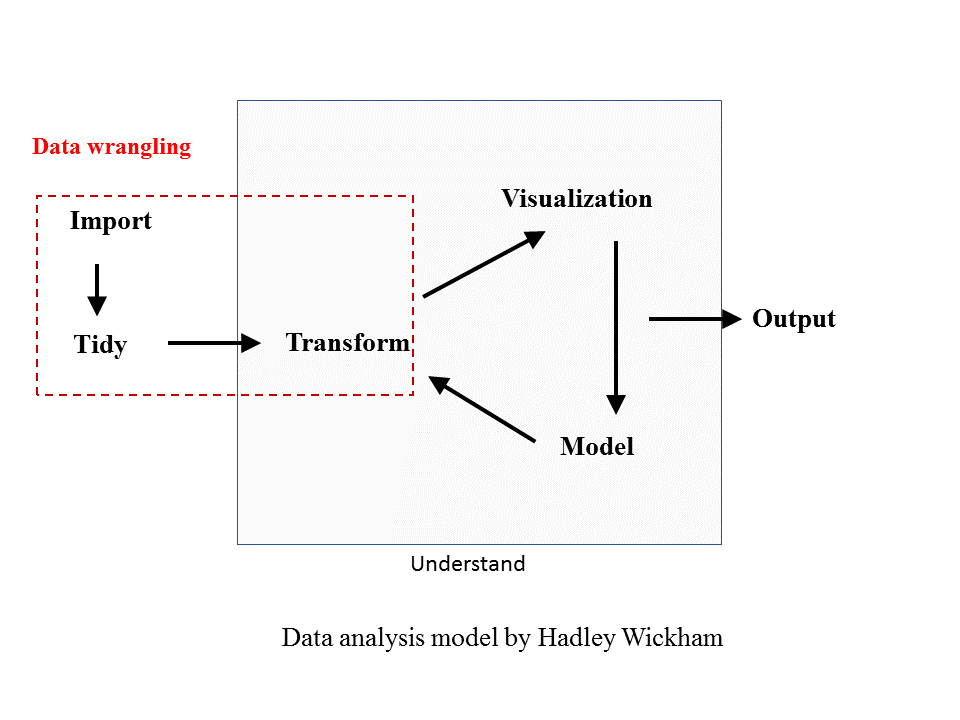
\includegraphics[width=1\linewidth]{img/DA_workflow} 

}

\caption{Data analysis workflow}\label{fig:figure2}
\end{figure}

\section{Data wrangling}\label{data-wrangling}

Data wrangling (see the above figure in red box) involves some basic
procedures (importing, tidying and transforming). R,and its packages,
\emph{tidyverse} in particular, provide a number of functions that can
help us deal with data cleaning and tranformation. We will be learning
how to use these functions in the follow sessions.

\chapter{Importing your data}\label{importing-your-data}

\section{from CSV/TXT}\label{from-csvtxt}

You can import data in csv (comma seperate) or text files that use a
different delimiter to seperate data. There two groups of functions you
can use:

\begin{itemize}
\item
  Base R functions
\item
  \emph{readr} package functions
\end{itemize}

\begin{center}\rule{0.5\linewidth}{\linethickness}\end{center}

\textbf{read.table( )} is a multipurpose function in R for importing
data, and this function has two special cases: \textbf{read.csv( )} and
\textbf{read.delim( )}.

\begin{itemize}
\item
  read.csv( ) is a wrapper for read.table with some default settings:
  sep = ``,'' ; header = TRUE.
\item
  read.delim( ) is a wrapper for read.table with some default settings:
  sep = ``\t'' ; header = TRUE.
\end{itemize}

\begin{center}\rule{0.5\linewidth}{\linethickness}\end{center}

\textbf{readr package} functions you need to \emph{library(readr)}

readr functions are 10 times faster than built-in functions.

\begin{itemize}
\tightlist
\item
  read\_csv( ): you can specify
\end{itemize}

\begin{quote}
col\_types = list(col\_double(), col\_character())
\end{quote}

\begin{quote}
col\_names = c(``a'',``b'')
\end{quote}

\begin{itemize}
\item
  read\_delim( )
\item
  read\_table( )
\end{itemize}

However, I found R-studio Import Dataset function most useful when
importing data. It offers an user interface and you will know how your
data look like when you choose different settings.

After R-studio inter face helps you import data initially, it is time
for us to take a look at what happens in the console.

You may want to copy the code automatically generated by R-Studio and
paste it in your script.

A little more about the path to directory: it is helpful to get to know
your working directory, you can get this information by \emph{getwd( )}.
When you know where you are, you can specify your folder either relative
to your present location or with the absolute path.

\begin{Shaded}
\begin{Highlighting}[]
\NormalTok{participant_}\DecValTok{1}\NormalTok{ <-}\StringTok{ }\KeywordTok{read.csv}\NormalTok{(}\StringTok{"data/participant_1.csv"}\NormalTok{)}
\CommentTok{#stringAsFactor = FALSE}

\NormalTok{participant_}\DecValTok{2}\NormalTok{ <-}\StringTok{ }\KeywordTok{read.csv}\NormalTok{(}\StringTok{"data/participant_2.csv"}\NormalTok{)}

\NormalTok{## from TXT}
\NormalTok{participant_1_tab <-}\StringTok{ }\KeywordTok{read.delim}\NormalTok{(}\StringTok{"~/OneDrive_Backup/OneDrive - Western Sydney University/JuqiangCHEN/310_Tutorial/DH_Data_wrangling/data/participant_1_tab.txt"}\NormalTok{)}
\end{Highlighting}
\end{Shaded}

\section{from EXCEL}\label{from-excel}

\begin{Shaded}
\begin{Highlighting}[]
\KeywordTok{library}\NormalTok{(readxl)}
\NormalTok{excel_test <-}\StringTok{ }\KeywordTok{read_excel}\NormalTok{(}\StringTok{"data/excel_test.xlsx"}\NormalTok{, }\DataTypeTok{sheet =} \StringTok{"participant_1"}\NormalTok{)}
\end{Highlighting}
\end{Shaded}

\section{Batch import}\label{batch-import}

\begin{Shaded}
\begin{Highlighting}[]
\KeywordTok{rbind}\NormalTok{(participant_}\DecValTok{1}\NormalTok{, participant_}\DecValTok{2}\NormalTok{)}

\NormalTok{all =}\StringTok{ }\KeywordTok{rbind}\NormalTok{(participant_}\DecValTok{1}\NormalTok{, participant_}\DecValTok{2}\NormalTok{)}

\CommentTok{# what about 10 more people?}

\NormalTok{participant_}\DecValTok{3}\NormalTok{ <-}\StringTok{ }\KeywordTok{read.csv}\NormalTok{(}\StringTok{"data/participant_3.csv"}\NormalTok{)}

\CommentTok{# get all the filenames of the folder}

\KeywordTok{getwd}\NormalTok{() }\CommentTok{# get working directory}

\KeywordTok{paste0}\NormalTok{(}\KeywordTok{getwd}\NormalTok{(), }\StringTok{"/data"}\NormalTok{) }\CommentTok{#specify the directory for the data}

\KeywordTok{list.files}\NormalTok{(}\KeywordTok{paste0}\NormalTok{(}\KeywordTok{getwd}\NormalTok{(), }\StringTok{"/data"}\NormalTok{),}\DataTypeTok{full.names=}\NormalTok{T) }\CommentTok{# full.names=T means getting the full path}

\NormalTok{filename =}\StringTok{ }\KeywordTok{list.files}\NormalTok{(}\KeywordTok{paste0}\NormalTok{(}\KeywordTok{getwd}\NormalTok{(), }\StringTok{"/data"}\NormalTok{),}\DataTypeTok{full.names=}\NormalTok{T, }\DataTypeTok{pattern =} \StringTok{".csv"}\NormalTok{) }\CommentTok{# get only csv files}

\CommentTok{# now you need a loop}
\NormalTok{df =}\StringTok{ }\KeywordTok{data.frame}\NormalTok{()}
\NormalTok{bin =}\StringTok{ }\KeywordTok{data.frame}\NormalTok{()}
\ControlFlowTok{for}\NormalTok{ (i }\ControlFlowTok{in} \DecValTok{1}\OperatorTok{:}\KeywordTok{length}\NormalTok{(filename))\{}
  \CommentTok{# length(filename) = how many files}
\NormalTok{  bin =}\StringTok{ }\KeywordTok{read.csv}\NormalTok{(filename[i])}
\NormalTok{  df =}\StringTok{ }\KeywordTok{rbind}\NormalTok{(df, bin)}
\NormalTok{\}}
\end{Highlighting}
\end{Shaded}

\section{Take a glimpse of the
dataframe}\label{take-a-glimpse-of-the-dataframe}

R has some basic functions that can help us have a quick look at the
data frame that we import.

\begin{itemize}
\tightlist
\item
  summary( )
\end{itemize}

1 For each factor variable, the levels are printed.

2 For each numeric variable, the minimun, first quantile, median, mean,
third quantile and the maximun values are shown.

\begin{itemize}
\tightlist
\item
  str( ) structure
\end{itemize}

This gives the information about the types of variables that your
dataframe contain.

Alternatively, you can hover your mouse over the head of the table, it
will give you basic information about the variable type of the column.

There are also other packages that offer data summer like the
\textbf{describe ( )}, similar to \textbf{summary ( )}, and
\textbf{contents ( )}, similar to \textbf{str ( )} in the Hmisc package.

\begin{Shaded}
\begin{Highlighting}[]
\KeywordTok{summary}\NormalTok{(all)}

\KeywordTok{str}\NormalTok{(all)}

\KeywordTok{library}\NormalTok{(Hmisc)}

\KeywordTok{describe}\NormalTok{(all)}

\KeywordTok{contents}\NormalTok{(all)}
\end{Highlighting}
\end{Shaded}

\chapter{Tidy your data}\label{tidy-your-data}

\section{what is tidy data?}\label{what-is-tidy-data}

Three rules:

\begin{itemize}
\item
  Each variable must have its own column.
\item
  Each observation must have its own row.
\item
  Each value must have its own cell.
\end{itemize}

\begin{Shaded}
\begin{Highlighting}[]
\KeywordTok{library}\NormalTok{(tidyverse)}
\KeywordTok{library}\NormalTok{(knitr)}
\CommentTok{# tidy data}
\KeywordTok{kable}\NormalTok{(table1, }\DataTypeTok{caption =} \StringTok{"a This is a tidy dataset!"}\NormalTok{)}
\end{Highlighting}
\end{Shaded}

\begin{table}[t]

\caption{\label{tab:unnamed-chunk-12}a This is a tidy dataset!}
\centering
\begin{tabular}{l|r|r|r}
\hline
country & year & cases & population\\
\hline
Afghanistan & 1999 & 745 & 19987071\\
\hline
Afghanistan & 2000 & 2666 & 20595360\\
\hline
Brazil & 1999 & 37737 & 172006362\\
\hline
Brazil & 2000 & 80488 & 174504898\\
\hline
China & 1999 & 212258 & 1272915272\\
\hline
China & 2000 & 213766 & 1280428583\\
\hline
\end{tabular}
\end{table}

\begin{Shaded}
\begin{Highlighting}[]
\KeywordTok{kable}\NormalTok{(table2, }\DataTypeTok{caption =} \StringTok{"b case and population missing"}\NormalTok{)}
\end{Highlighting}
\end{Shaded}

\begin{table}[t]

\caption{\label{tab:unnamed-chunk-12}b case and population missing}
\centering
\begin{tabular}{l|r|l|r}
\hline
country & year & type & count\\
\hline
Afghanistan & 1999 & cases & 745\\
\hline
Afghanistan & 1999 & population & 19987071\\
\hline
Afghanistan & 2000 & cases & 2666\\
\hline
Afghanistan & 2000 & population & 20595360\\
\hline
Brazil & 1999 & cases & 37737\\
\hline
Brazil & 1999 & population & 172006362\\
\hline
Brazil & 2000 & cases & 80488\\
\hline
Brazil & 2000 & population & 174504898\\
\hline
China & 1999 & cases & 212258\\
\hline
China & 1999 & population & 1272915272\\
\hline
China & 2000 & cases & 213766\\
\hline
China & 2000 & population & 1280428583\\
\hline
\end{tabular}
\end{table}

\begin{Shaded}
\begin{Highlighting}[]
\KeywordTok{kable}\NormalTok{(table3, }\DataTypeTok{caption =} \StringTok{"c case and population merged"}\NormalTok{)}
\end{Highlighting}
\end{Shaded}

\begin{table}[t]

\caption{\label{tab:unnamed-chunk-12}c case and population merged}
\centering
\begin{tabular}{l|r|l}
\hline
country & year & rate\\
\hline
Afghanistan & 1999 & 745/19987071\\
\hline
Afghanistan & 2000 & 2666/20595360\\
\hline
Brazil & 1999 & 37737/172006362\\
\hline
Brazil & 2000 & 80488/174504898\\
\hline
China & 1999 & 212258/1272915272\\
\hline
China & 2000 & 213766/1280428583\\
\hline
\end{tabular}
\end{table}

\begin{Shaded}
\begin{Highlighting}[]
\KeywordTok{kable}\NormalTok{(table4a, }\DataTypeTok{caption =} \StringTok{"d year missing, cases"}\NormalTok{)}
\end{Highlighting}
\end{Shaded}

\begin{table}[t]

\caption{\label{tab:unnamed-chunk-12}d year missing, cases}
\centering
\begin{tabular}{l|r|r}
\hline
country & 1999 & 2000\\
\hline
Afghanistan & 745 & 2666\\
\hline
Brazil & 37737 & 80488\\
\hline
China & 212258 & 213766\\
\hline
\end{tabular}
\end{table}

\begin{Shaded}
\begin{Highlighting}[]
\KeywordTok{kable}\NormalTok{(table4b, }\DataTypeTok{caption =} \StringTok{"e year missing, population"}\NormalTok{)}
\end{Highlighting}
\end{Shaded}

\begin{table}[t]

\caption{\label{tab:unnamed-chunk-12}e year missing, population}
\centering
\begin{tabular}{l|r|r}
\hline
country & 1999 & 2000\\
\hline
Afghanistan & 19987071 & 20595360\\
\hline
Brazil & 172006362 & 174504898\\
\hline
China & 1272915272 & 1280428583\\
\hline
\end{tabular}
\end{table}

\section{Tools in tidyr}\label{tools-in-tidyr}

\subsection{gather ( )}\label{gather}

For some datasets, some of the column names are not names of variables
but \textbf{values} of a variable.

\begin{Shaded}
\begin{Highlighting}[]
\KeywordTok{kable}\NormalTok{(table4a, }\DataTypeTok{caption=} \StringTok{"year missing, cases"}\NormalTok{)}
\end{Highlighting}
\end{Shaded}

\begin{table}[t]

\caption{\label{tab:unnamed-chunk-13}year missing, cases}
\centering
\begin{tabular}{l|r|r}
\hline
country & 1999 & 2000\\
\hline
Afghanistan & 745 & 2666\\
\hline
Brazil & 37737 & 80488\\
\hline
China & 212258 & 213766\\
\hline
\end{tabular}
\end{table}

We need to gather years like 1999 and 2000 into one variable
\textbf{year}.

\begin{Shaded}
\begin{Highlighting}[]
\KeywordTok{gather}\NormalTok{(table4a, }\StringTok{'1999'}\NormalTok{,}\StringTok{'2000'}\NormalTok{,}\DataTypeTok{key =} \StringTok{"year"}\NormalTok{, }\DataTypeTok{value =} \StringTok{"cases"}\NormalTok{)}
\end{Highlighting}
\end{Shaded}

\begin{verbatim}
## # A tibble: 6 x 3
##   country     year   cases
##   <chr>       <chr>  <int>
## 1 Afghanistan 1999     745
## 2 Brazil      1999   37737
## 3 China       1999  212258
## 4 Afghanistan 2000    2666
## 5 Brazil      2000   80488
## 6 China       2000  213766
\end{verbatim}

\begin{Shaded}
\begin{Highlighting}[]
\KeywordTok{gather}\NormalTok{(table4b, }\StringTok{'1999'}\NormalTok{,}\StringTok{'2000'}\NormalTok{,}\DataTypeTok{key =} \StringTok{"year"}\NormalTok{, }\DataTypeTok{value =} \StringTok{"population"}\NormalTok{)}
\end{Highlighting}
\end{Shaded}

\begin{verbatim}
## # A tibble: 6 x 3
##   country     year  population
##   <chr>       <chr>      <int>
## 1 Afghanistan 1999    19987071
## 2 Brazil      1999   172006362
## 3 China       1999  1272915272
## 4 Afghanistan 2000    20595360
## 5 Brazil      2000   174504898
## 6 China       2000  1280428583
\end{verbatim}

\subsection{spread ( )}\label{spread}

Sometime the observations are scattered across muiltiple rows.

\begin{Shaded}
\begin{Highlighting}[]
\KeywordTok{kable}\NormalTok{(table2, }\DataTypeTok{caption =} \StringTok{"b case and population missing"}\NormalTok{)}
\end{Highlighting}
\end{Shaded}

\begin{table}[t]

\caption{\label{tab:unnamed-chunk-15}b case and population missing}
\centering
\begin{tabular}{l|r|l|r}
\hline
country & year & type & count\\
\hline
Afghanistan & 1999 & cases & 745\\
\hline
Afghanistan & 1999 & population & 19987071\\
\hline
Afghanistan & 2000 & cases & 2666\\
\hline
Afghanistan & 2000 & population & 20595360\\
\hline
Brazil & 1999 & cases & 37737\\
\hline
Brazil & 1999 & population & 172006362\\
\hline
Brazil & 2000 & cases & 80488\\
\hline
Brazil & 2000 & population & 174504898\\
\hline
China & 1999 & cases & 212258\\
\hline
China & 1999 & population & 1272915272\\
\hline
China & 2000 & cases & 213766\\
\hline
China & 2000 & population & 1280428583\\
\hline
\end{tabular}
\end{table}

\begin{Shaded}
\begin{Highlighting}[]
\KeywordTok{spread}\NormalTok{(table2, }\DataTypeTok{key =}\NormalTok{ type, }\DataTypeTok{value =}\NormalTok{ count)}
\end{Highlighting}
\end{Shaded}

\begin{verbatim}
## # A tibble: 6 x 4
##   country      year  cases population
##   <chr>       <int>  <int>      <int>
## 1 Afghanistan  1999    745   19987071
## 2 Afghanistan  2000   2666   20595360
## 3 Brazil       1999  37737  172006362
## 4 Brazil       2000  80488  174504898
## 5 China        1999 212258 1272915272
## 6 China        2000 213766 1280428583
\end{verbatim}

To sum up, gather() makes wide tables long while spread() makes long
tables wide. The key idea here is to think about the variables you want
to explore and make sure that they are placed in different columns. This
is very important for data visualization and stats modeling in R.

\begin{center}\rule{0.5\linewidth}{\linethickness}\end{center}

\subsection{separate()}\label{separate}

In some cases, one column may contain a combination of two variables. We
need to separate these two variables.

\begin{Shaded}
\begin{Highlighting}[]
\KeywordTok{kable}\NormalTok{(table3, }\DataTypeTok{caption =} \StringTok{"c case and population merged"}\NormalTok{)}
\end{Highlighting}
\end{Shaded}

\begin{table}[t]

\caption{\label{tab:unnamed-chunk-16}c case and population merged}
\centering
\begin{tabular}{l|r|l}
\hline
country & year & rate\\
\hline
Afghanistan & 1999 & 745/19987071\\
\hline
Afghanistan & 2000 & 2666/20595360\\
\hline
Brazil & 1999 & 37737/172006362\\
\hline
Brazil & 2000 & 80488/174504898\\
\hline
China & 1999 & 212258/1272915272\\
\hline
China & 2000 & 213766/1280428583\\
\hline
\end{tabular}
\end{table}

\begin{Shaded}
\begin{Highlighting}[]
\CommentTok{#separate by a delimiter}
\KeywordTok{separate}\NormalTok{(table3, rate, }\DataTypeTok{into =} \KeywordTok{c}\NormalTok{(}\StringTok{"cases"}\NormalTok{, }\StringTok{"population"}\NormalTok{), }\DataTypeTok{sep =} \StringTok{"/"}\NormalTok{)}
\end{Highlighting}
\end{Shaded}

\begin{verbatim}
## # A tibble: 6 x 4
##   country      year cases  population
##   <chr>       <int> <chr>  <chr>     
## 1 Afghanistan  1999 745    19987071  
## 2 Afghanistan  2000 2666   20595360  
## 3 Brazil       1999 37737  172006362 
## 4 Brazil       2000 80488  174504898 
## 5 China        1999 212258 1272915272
## 6 China        2000 213766 1280428583
\end{verbatim}

\begin{Shaded}
\begin{Highlighting}[]
\CommentTok{#separate by the first two digits}

\KeywordTok{separate}\NormalTok{(table3, rate, }\DataTypeTok{into =} \KeywordTok{c}\NormalTok{(}\StringTok{"cases"}\NormalTok{, }\StringTok{"population"}\NormalTok{), }\DataTypeTok{sep =} \DecValTok{2}\NormalTok{)}
\end{Highlighting}
\end{Shaded}

\begin{verbatim}
## # A tibble: 6 x 4
##   country      year cases population     
##   <chr>       <int> <chr> <chr>          
## 1 Afghanistan  1999 74    5/19987071     
## 2 Afghanistan  2000 26    66/20595360    
## 3 Brazil       1999 37    737/172006362  
## 4 Brazil       2000 80    488/174504898  
## 5 China        1999 21    2258/1272915272
## 6 China        2000 21    3766/1280428583
\end{verbatim}

\begin{Shaded}
\begin{Highlighting}[]
\CommentTok{#separate by the last two digits}

\KeywordTok{separate}\NormalTok{(table3, rate, }\DataTypeTok{into =} \KeywordTok{c}\NormalTok{(}\StringTok{"cases"}\NormalTok{, }\StringTok{"population"}\NormalTok{), }\DataTypeTok{sep =} \OperatorTok{-}\DecValTok{2}\NormalTok{)}
\end{Highlighting}
\end{Shaded}

\begin{verbatim}
## # A tibble: 6 x 4
##   country      year cases           population
##   <chr>       <int> <chr>           <chr>     
## 1 Afghanistan  1999 745/199870      71        
## 2 Afghanistan  2000 2666/205953     60        
## 3 Brazil       1999 37737/1720063   62        
## 4 Brazil       2000 80488/1745048   98        
## 5 China        1999 212258/12729152 72        
## 6 China        2000 213766/12804285 83
\end{verbatim}

\subsection{unite()}\label{unite}

\begin{Shaded}
\begin{Highlighting}[]
\NormalTok{table_new =}\StringTok{ }\KeywordTok{separate}\NormalTok{(table3, year, }\DataTypeTok{into =} \KeywordTok{c}\NormalTok{(}\StringTok{"year1"}\NormalTok{, }\StringTok{"year2"}\NormalTok{), }\DataTypeTok{sep =} \DecValTok{2}\NormalTok{)}

\NormalTok{table_new}
\end{Highlighting}
\end{Shaded}

\begin{verbatim}
## # A tibble: 6 x 4
##   country     year1 year2 rate             
##   <chr>       <chr> <chr> <chr>            
## 1 Afghanistan 19    99    745/19987071     
## 2 Afghanistan 20    00    2666/20595360    
## 3 Brazil      19    99    37737/172006362  
## 4 Brazil      20    00    80488/174504898  
## 5 China       19    99    212258/1272915272
## 6 China       20    00    213766/1280428583
\end{verbatim}

\begin{Shaded}
\begin{Highlighting}[]
\KeywordTok{unite}\NormalTok{(table_new, new, year1, year2)}\CommentTok{# by default there is an underscore between two parts.}
\end{Highlighting}
\end{Shaded}

\begin{verbatim}
## # A tibble: 6 x 3
##   country     new   rate             
##   <chr>       <chr> <chr>            
## 1 Afghanistan 19_99 745/19987071     
## 2 Afghanistan 20_00 2666/20595360    
## 3 Brazil      19_99 37737/172006362  
## 4 Brazil      20_00 80488/174504898  
## 5 China       19_99 212258/1272915272
## 6 China       20_00 213766/1280428583
\end{verbatim}

\begin{Shaded}
\begin{Highlighting}[]
\KeywordTok{unite}\NormalTok{(table_new, new, year1, year2, }\DataTypeTok{sep =} \StringTok{""}\NormalTok{)}
\end{Highlighting}
\end{Shaded}

\begin{verbatim}
## # A tibble: 6 x 3
##   country     new   rate             
##   <chr>       <chr> <chr>            
## 1 Afghanistan 1999  745/19987071     
## 2 Afghanistan 2000  2666/20595360    
## 3 Brazil      1999  37737/172006362  
## 4 Brazil      2000  80488/174504898  
## 5 China       1999  212258/1272915272
## 6 China       2000  213766/1280428583
\end{verbatim}

\chapter{Tranform your data}\label{tranform-your-data}

\section{Selecting variables of
interest}\label{selecting-variables-of-interest}

When we get a dataset, one of the most important things to do is to pick
the variables we need, especially when the raw dataset has too many
columns.

\begin{Shaded}
\begin{Highlighting}[]
\KeywordTok{library}\NormalTok{(tidyverse)}

\CommentTok{# getting the data}
\NormalTok{filename =}\StringTok{ }\KeywordTok{list.files}\NormalTok{(}\KeywordTok{paste0}\NormalTok{(}\KeywordTok{getwd}\NormalTok{(), }\StringTok{"/data"}\NormalTok{),}\DataTypeTok{full.names=}\NormalTok{T, }\DataTypeTok{pattern =} \StringTok{".csv"}\NormalTok{) }\CommentTok{# get only csv files}

\NormalTok{df =}\StringTok{ }\KeywordTok{data.frame}\NormalTok{()}
\NormalTok{bin =}\StringTok{ }\KeywordTok{data.frame}\NormalTok{()}
\ControlFlowTok{for}\NormalTok{ (i }\ControlFlowTok{in} \DecValTok{1}\OperatorTok{:}\KeywordTok{length}\NormalTok{(filename))\{}
  \CommentTok{# length(filename) = how many files}
\NormalTok{  bin =}\StringTok{ }\KeywordTok{read.csv}\NormalTok{(filename[i])}
\NormalTok{  df =}\StringTok{ }\KeywordTok{rbind}\NormalTok{(df, bin)}
\NormalTok{\}}

\CommentTok{#head(df)}

\CommentTok{#colnames(df)}
\end{Highlighting}
\end{Shaded}

In this dataset \emph{df}, we need to get the \emph{ID} of participants
as stored in Subject, the \emph{stimuli} they heard in ``tone.Trial'',
their \emph{response} in ``insex1.RESP'', their \emph{response time} in
``insex1.RT'', and the \emph{experiment conditions} in
``Procedure.Block.''.

\begin{Shaded}
\begin{Highlighting}[]
\NormalTok{df_new =}\StringTok{ }\KeywordTok{select}\NormalTok{(df, }\DataTypeTok{subject =} \StringTok{"Subject"}\NormalTok{,}
                \DataTypeTok{stimuli =} \StringTok{"tone.Trial."}\NormalTok{,}
                \DataTypeTok{response =} \StringTok{"insex1.RESP"}\NormalTok{,}
                \DataTypeTok{response_rt =} \StringTok{"insex1.RT"}\NormalTok{,}
                \DataTypeTok{block =} \StringTok{"Procedure.Block."}\NormalTok{,}
\NormalTok{                ExperimentName)}
\KeywordTok{head}\NormalTok{(df_new)}
\end{Highlighting}
\end{Shaded}

\begin{verbatim}
##   subject stimuli response response_rt    block           ExperimentName
## 1     402      NA                   NA pracproc Assim_main_chinese_500ms
## 2     402      NA                   NA pracproc Assim_main_chinese_500ms
## 3     402      NA                   NA pracproc Assim_main_chinese_500ms
## 4     402      NA                   NA pracproc Assim_main_chinese_500ms
## 5     402      NA                   NA pracproc Assim_main_chinese_500ms
## 6     402      NA                   NA pracproc Assim_main_chinese_500ms
\end{verbatim}

\begin{Shaded}
\begin{Highlighting}[]
\CommentTok{# select by names}
\KeywordTok{head}\NormalTok{(}\KeywordTok{select}\NormalTok{(df_new, subject}\OperatorTok{:}\StringTok{ }\NormalTok{response))}
\end{Highlighting}
\end{Shaded}

\begin{verbatim}
##   subject stimuli response
## 1     402      NA         
## 2     402      NA         
## 3     402      NA         
## 4     402      NA         
## 5     402      NA         
## 6     402      NA
\end{verbatim}

\begin{Shaded}
\begin{Highlighting}[]
\KeywordTok{head}\NormalTok{(}\KeywordTok{select}\NormalTok{(df_new, subject}\OperatorTok{:}\StringTok{ }\NormalTok{response))}
\end{Highlighting}
\end{Shaded}

\begin{verbatim}
##   subject stimuli response
## 1     402      NA         
## 2     402      NA         
## 3     402      NA         
## 4     402      NA         
## 5     402      NA         
## 6     402      NA
\end{verbatim}

\begin{Shaded}
\begin{Highlighting}[]
\KeywordTok{head}\NormalTok{(}\KeywordTok{select}\NormalTok{(df_new, }\DecValTok{1}\OperatorTok{:}\StringTok{ }\DecValTok{3}\NormalTok{))}
\end{Highlighting}
\end{Shaded}

\begin{verbatim}
##   subject stimuli response
## 1     402      NA         
## 2     402      NA         
## 3     402      NA         
## 4     402      NA         
## 5     402      NA         
## 6     402      NA
\end{verbatim}

\begin{Shaded}
\begin{Highlighting}[]
\KeywordTok{head}\NormalTok{(}\KeywordTok{select}\NormalTok{(df_new, }\OperatorTok{-}\NormalTok{subject))}
\end{Highlighting}
\end{Shaded}

\begin{verbatim}
##   stimuli response response_rt    block           ExperimentName
## 1      NA                   NA pracproc Assim_main_chinese_500ms
## 2      NA                   NA pracproc Assim_main_chinese_500ms
## 3      NA                   NA pracproc Assim_main_chinese_500ms
## 4      NA                   NA pracproc Assim_main_chinese_500ms
## 5      NA                   NA pracproc Assim_main_chinese_500ms
## 6      NA                   NA pracproc Assim_main_chinese_500ms
\end{verbatim}

\begin{Shaded}
\begin{Highlighting}[]
\KeywordTok{head}\NormalTok{(}\KeywordTok{select}\NormalTok{(df_new, ExperimentName, }\KeywordTok{everything}\NormalTok{()))}
\end{Highlighting}
\end{Shaded}

\begin{verbatim}
##             ExperimentName subject stimuli response response_rt    block
## 1 Assim_main_chinese_500ms     402      NA                   NA pracproc
## 2 Assim_main_chinese_500ms     402      NA                   NA pracproc
## 3 Assim_main_chinese_500ms     402      NA                   NA pracproc
## 4 Assim_main_chinese_500ms     402      NA                   NA pracproc
## 5 Assim_main_chinese_500ms     402      NA                   NA pracproc
## 6 Assim_main_chinese_500ms     402      NA                   NA pracproc
\end{verbatim}

\begin{Shaded}
\begin{Highlighting}[]
\CommentTok{# change column names}

\KeywordTok{head}\NormalTok{(}\KeywordTok{rename}\NormalTok{(df_new, }\DataTypeTok{exp =}\NormalTok{ ExperimentName))}
\end{Highlighting}
\end{Shaded}

\begin{verbatim}
##   subject stimuli response response_rt    block                      exp
## 1     402      NA                   NA pracproc Assim_main_chinese_500ms
## 2     402      NA                   NA pracproc Assim_main_chinese_500ms
## 3     402      NA                   NA pracproc Assim_main_chinese_500ms
## 4     402      NA                   NA pracproc Assim_main_chinese_500ms
## 5     402      NA                   NA pracproc Assim_main_chinese_500ms
## 6     402      NA                   NA pracproc Assim_main_chinese_500ms
\end{verbatim}

\section{Filtering observations}\label{filtering-observations}

Not all the data in the raw dataset are useful. We can use filter( )
function to select rows or observations based on some criteria.

Three useful logical operators for forming conditions:

\begin{itemize}
\item
  \textbf{\&} means ``and''
\item
  \textbf{\textbar{}} means ``or''
\item
  \textbf{!} means ``not''
\end{itemize}

\begin{Shaded}
\begin{Highlighting}[]
\CommentTok{# removing data from the practice block}
\NormalTok{df_new =}\StringTok{ }\KeywordTok{filter}\NormalTok{(df_new, block }\OperatorTok{!=}\StringTok{ "pracproc"}\NormalTok{)}
\KeywordTok{head}\NormalTok{(df_new)}
\end{Highlighting}
\end{Shaded}

\begin{verbatim}
##   subject stimuli response response_rt  block           ExperimentName
## 1     402      33        f         672 block6 Assim_main_chinese_500ms
## 2     402     315        j        2831 block6 Assim_main_chinese_500ms
## 3     402      45                    0 block6 Assim_main_chinese_500ms
## 4     402      21                    0 block6 Assim_main_chinese_500ms
## 5     402      33        f        1041 block6 Assim_main_chinese_500ms
## 6     402     241                    0 block6 Assim_main_chinese_500ms
\end{verbatim}

\begin{Shaded}
\begin{Highlighting}[]
\CommentTok{# removing missing data in response column}
\NormalTok{df_new =}\StringTok{ }\KeywordTok{filter}\NormalTok{(df_new, }\OperatorTok{!}\KeywordTok{is.na}\NormalTok{(response))}
\NormalTok{df_new =}\StringTok{ }\KeywordTok{filter}\NormalTok{(df_new, response }\OperatorTok{!=}\StringTok{ ""}\NormalTok{)}
\KeywordTok{head}\NormalTok{(df_new)}
\end{Highlighting}
\end{Shaded}

\begin{verbatim}
##   subject stimuli response response_rt  block           ExperimentName
## 1     402      33        f         672 block6 Assim_main_chinese_500ms
## 2     402     315        j        2831 block6 Assim_main_chinese_500ms
## 3     402      33        f        1041 block6 Assim_main_chinese_500ms
## 4     402     315        j         363 block6 Assim_main_chinese_500ms
## 5     402      21        f        1234 block6 Assim_main_chinese_500ms
## 6     402      45        j         322 block6 Assim_main_chinese_500ms
\end{verbatim}

\begin{Shaded}
\begin{Highlighting}[]
\CommentTok{# pick up stimuli 33 and 21}

\KeywordTok{head}\NormalTok{(}\KeywordTok{filter}\NormalTok{(df_new, stimuli }\OperatorTok{==}\StringTok{ }\DecValTok{33} \OperatorTok{|}\StringTok{ }\NormalTok{stimuli }\OperatorTok{==}\StringTok{ }\DecValTok{21}\NormalTok{))}
\end{Highlighting}
\end{Shaded}

\begin{verbatim}
##   subject stimuli response response_rt  block           ExperimentName
## 1     402      33        f         672 block6 Assim_main_chinese_500ms
## 2     402      33        f        1041 block6 Assim_main_chinese_500ms
## 3     402      21        f        1234 block6 Assim_main_chinese_500ms
## 4     402      33        f         150 block6 Assim_main_chinese_500ms
## 5     402      33        f         206 block6 Assim_main_chinese_500ms
## 6     402      21        f          52 block6 Assim_main_chinese_500ms
\end{verbatim}

\begin{Shaded}
\begin{Highlighting}[]
\KeywordTok{head}\NormalTok{(}\KeywordTok{filter}\NormalTok{(df_new, stimuli }\OperatorTok\StringTok{ }\KeywordTok{c}\NormalTok{(}\DecValTok{33}\NormalTok{, }\DecValTok{21}\NormalTok{)))}
\end{Highlighting}
\end{Shaded}

\begin{verbatim}
##   subject stimuli response response_rt  block           ExperimentName
## 1     402      33        f         672 block6 Assim_main_chinese_500ms
## 2     402      33        f        1041 block6 Assim_main_chinese_500ms
## 3     402      21        f        1234 block6 Assim_main_chinese_500ms
## 4     402      33        f         150 block6 Assim_main_chinese_500ms
## 5     402      33        f         206 block6 Assim_main_chinese_500ms
## 6     402      21        f          52 block6 Assim_main_chinese_500ms
\end{verbatim}

\begin{Shaded}
\begin{Highlighting}[]
\CommentTok{# removing data with respones time shorter than 200}

\KeywordTok{head}\NormalTok{(}\KeywordTok{filter}\NormalTok{(df_new, response_rt }\OperatorTok{<}\StringTok{ }\DecValTok{200}\NormalTok{))}
\end{Highlighting}
\end{Shaded}

\begin{verbatim}
##   subject stimuli response response_rt  block           ExperimentName
## 1     402      45        j         109 block6 Assim_main_chinese_500ms
## 2     402      33        f         150 block6 Assim_main_chinese_500ms
## 3     402      21        f          52 block6 Assim_main_chinese_500ms
## 4     402      33        f         107 block5 Assim_main_chinese_500ms
## 5     402      33        f         153 block5 Assim_main_chinese_500ms
## 6     402      21        f          95 block2 Assim_main_chinese_500ms
\end{verbatim}

\begin{Shaded}
\begin{Highlighting}[]
\KeywordTok{head}\NormalTok{(}\KeywordTok{filter}\NormalTok{(df_new, response_rt }\OperatorTok{>}\StringTok{ }\DecValTok{200}\NormalTok{))}
\end{Highlighting}
\end{Shaded}

\begin{verbatim}
##   subject stimuli response response_rt  block           ExperimentName
## 1     402      33        f         672 block6 Assim_main_chinese_500ms
## 2     402     315        j        2831 block6 Assim_main_chinese_500ms
## 3     402      33        f        1041 block6 Assim_main_chinese_500ms
## 4     402     315        j         363 block6 Assim_main_chinese_500ms
## 5     402      21        f        1234 block6 Assim_main_chinese_500ms
## 6     402      45        j         322 block6 Assim_main_chinese_500ms
\end{verbatim}

\section{Changing the order of rows}\label{changing-the-order-of-rows}

\begin{Shaded}
\begin{Highlighting}[]
\CommentTok{# arrange the dataframe by stimuli and response_rt columns}
\KeywordTok{head}\NormalTok{(}\KeywordTok{arrange}\NormalTok{(df_new, stimuli, response_rt))}
\end{Highlighting}
\end{Shaded}

\begin{verbatim}
##   subject stimuli response response_rt  block              ExperimentName
## 1     418      21        g           6 block7 assim_main_vietnamese_500ms
## 2     418      21        g          51 block4 assim_main_vietnamese_500ms
## 3     402      21        f          52 block6    Assim_main_chinese_500ms
## 4     418      21        g          85 block1 assim_main_vietnamese_500ms
## 5     402      21        f          95 block2    Assim_main_chinese_500ms
## 6     418      21        g          99 block7 assim_main_vietnamese_500ms
\end{verbatim}

\begin{Shaded}
\begin{Highlighting}[]
\CommentTok{# arrange the dataframe by stimuli and the descending order of block columns}
\KeywordTok{head}\NormalTok{(}\KeywordTok{arrange}\NormalTok{(df_new, stimuli, }\KeywordTok{desc}\NormalTok{(block)))}
\end{Highlighting}
\end{Shaded}

\begin{verbatim}
##   subject stimuli response response_rt  block              ExperimentName
## 1     402      21        f         609 block7    Assim_main_chinese_500ms
## 2     402      21        f         224 block7    Assim_main_chinese_500ms
## 3     402      21        f         286 block7    Assim_main_chinese_500ms
## 4     402      21        f        1136 block7    Assim_main_chinese_500ms
## 5     418      21        g           6 block7 assim_main_vietnamese_500ms
## 6     418      21        g         331 block7 assim_main_vietnamese_500ms
\end{verbatim}

\section{Generating new variables}\label{generating-new-variables}

We can generate new variables based on existing variables using the
function mutate() and transmutate(). The difference is mutate will keep
the original variables while transmutate will erase orginal variables.

\begin{Shaded}
\begin{Highlighting}[]
\CommentTok{# you can add, minus, log transform any numberic column}
\KeywordTok{head}\NormalTok{(}\KeywordTok{mutate}\NormalTok{(df_new, }\DataTypeTok{response_rt_new =} \KeywordTok{log}\NormalTok{(response_rt)))}
\end{Highlighting}
\end{Shaded}

\begin{verbatim}
##   subject stimuli response response_rt  block           ExperimentName
## 1     402      33        f         672 block6 Assim_main_chinese_500ms
## 2     402     315        j        2831 block6 Assim_main_chinese_500ms
## 3     402      33        f        1041 block6 Assim_main_chinese_500ms
## 4     402     315        j         363 block6 Assim_main_chinese_500ms
## 5     402      21        f        1234 block6 Assim_main_chinese_500ms
## 6     402      45        j         322 block6 Assim_main_chinese_500ms
##   response_rt_new
## 1        6.510258
## 2        7.948385
## 3        6.947937
## 4        5.894403
## 5        7.118016
## 6        5.774552
\end{verbatim}

\begin{Shaded}
\begin{Highlighting}[]
\CommentTok{# you can extract part of the information from a character variable}

\KeywordTok{head}\NormalTok{(}\KeywordTok{mutate}\NormalTok{(df_new, }\DataTypeTok{ISI =} \KeywordTok{str_extract}\NormalTok{(ExperimentName, }\StringTok{"2000|500"}\NormalTok{)))}
\end{Highlighting}
\end{Shaded}

\begin{verbatim}
##   subject stimuli response response_rt  block           ExperimentName ISI
## 1     402      33        f         672 block6 Assim_main_chinese_500ms 500
## 2     402     315        j        2831 block6 Assim_main_chinese_500ms 500
## 3     402      33        f        1041 block6 Assim_main_chinese_500ms 500
## 4     402     315        j         363 block6 Assim_main_chinese_500ms 500
## 5     402      21        f        1234 block6 Assim_main_chinese_500ms 500
## 6     402      45        j         322 block6 Assim_main_chinese_500ms 500
\end{verbatim}

\begin{Shaded}
\begin{Highlighting}[]
\KeywordTok{head}\NormalTok{(}\KeywordTok{transmute}\NormalTok{(df_new, }\DataTypeTok{ISI =} \KeywordTok{str_extract}\NormalTok{(ExperimentName, }\StringTok{"2000|500"}\NormalTok{)))}
\end{Highlighting}
\end{Shaded}

\begin{verbatim}
##   ISI
## 1 500
## 2 500
## 3 500
## 4 500
## 5 500
## 6 500
\end{verbatim}

\begin{Shaded}
\begin{Highlighting}[]
\CommentTok{# you can paste two variabls together}

\KeywordTok{head}\NormalTok{(}\KeywordTok{transmute}\NormalTok{(df_new, }\DataTypeTok{ISI =} \KeywordTok{paste}\NormalTok{(stimuli, block, }\DataTypeTok{sep =} \StringTok{"_"}\NormalTok{)))}
\end{Highlighting}
\end{Shaded}

\begin{verbatim}
##          ISI
## 1  33_block6
## 2 315_block6
## 3  33_block6
## 4 315_block6
## 5  21_block6
## 6  45_block6
\end{verbatim}

\begin{Shaded}
\begin{Highlighting}[]
\CommentTok{# you can recode a variable}

\KeywordTok{head}\NormalTok{( }\KeywordTok{mutate}\NormalTok{(df_new, }\DataTypeTok{block =} \KeywordTok{recode}\NormalTok{(block, }
                         \DataTypeTok{block1 =} \StringTok{"ss"}\NormalTok{, }\DataTypeTok{block2 =} \StringTok{"ss"}\NormalTok{,}
                         \DataTypeTok{block3 =} \StringTok{"sd"}\NormalTok{, }\DataTypeTok{block4 =} \StringTok{"sd"}\NormalTok{,}
                         \DataTypeTok{block5 =} \StringTok{"ds"}\NormalTok{, }\DataTypeTok{block6 =} \StringTok{"ds"}\NormalTok{,}
                         \DataTypeTok{block7 =} \StringTok{"dd"}\NormalTok{)))}
\end{Highlighting}
\end{Shaded}

\begin{verbatim}
##   subject stimuli response response_rt block           ExperimentName
## 1     402      33        f         672    ds Assim_main_chinese_500ms
## 2     402     315        j        2831    ds Assim_main_chinese_500ms
## 3     402      33        f        1041    ds Assim_main_chinese_500ms
## 4     402     315        j         363    ds Assim_main_chinese_500ms
## 5     402      21        f        1234    ds Assim_main_chinese_500ms
## 6     402      45        j         322    ds Assim_main_chinese_500ms
\end{verbatim}

\section{\texorpdfstring{The pipeline
``\%\textgreater{}\%''}{The pipeline \%\textgreater{}\%}}\label{the-pipeline}

You may have noticed the repetition in the above codes. We have to
specify the dataframe every time we use a function and have to store it
in a new name if we want to keep the original dataframe.

Using pipeline \emph{\%\textgreater{}\%} can reduce the redundancy and
the mistake we may make when we have a dozen of dataframes to refer to.

\begin{Shaded}
\begin{Highlighting}[]
\NormalTok{df_final =}\StringTok{ }\NormalTok{df }\OperatorTok
\StringTok{  }\CommentTok{# selecting the columns we need}
\StringTok{  }\KeywordTok{select}\NormalTok{(., }\DataTypeTok{subject =} \StringTok{"Subject"}\NormalTok{,}
                \DataTypeTok{stimuli =} \StringTok{"tone.Trial."}\NormalTok{,}
                \DataTypeTok{response =} \StringTok{"insex1.RESP"}\NormalTok{,}
                \DataTypeTok{response_rt =} \StringTok{"insex1.RT"}\NormalTok{,}
                \DataTypeTok{block =} \StringTok{"Procedure.Block."}\NormalTok{,}
                \DataTypeTok{exp =}\NormalTok{ ExperimentName)}\OperatorTok
\StringTok{  }\CommentTok{#filtering out useless data}
\StringTok{  }\KeywordTok{filter}\NormalTok{(block }\OperatorTok{!=}\StringTok{ "pracproc"} \OperatorTok{&}\StringTok{ }\OperatorTok{!}\KeywordTok{is.na}\NormalTok{(response) }\OperatorTok{&}\StringTok{ }\NormalTok{response }\OperatorTok{!=}\StringTok{ ""}\NormalTok{)}\OperatorTok
\StringTok{  }\CommentTok{# generating new variables based on old variables}
\StringTok{  }\KeywordTok{mutate}\NormalTok{(}\DataTypeTok{ISI =} \KeywordTok{str_extract}\NormalTok{(exp, }\StringTok{"2000|500"}\NormalTok{),}
         \DataTypeTok{block =} \KeywordTok{recode}\NormalTok{(block, }
                         \DataTypeTok{block1 =} \StringTok{"ss"}\NormalTok{, }\DataTypeTok{block2 =} \StringTok{"ss"}\NormalTok{,}
                         \DataTypeTok{block3 =} \StringTok{"sd"}\NormalTok{, }\DataTypeTok{block4 =} \StringTok{"sd"}\NormalTok{,}
                         \DataTypeTok{block5 =} \StringTok{"ds"}\NormalTok{, }\DataTypeTok{block6 =} \StringTok{"ds"}\NormalTok{,}
                         \DataTypeTok{block7 =} \StringTok{"dd"}\NormalTok{))}
\end{Highlighting}
\end{Shaded}

\section{Summarizing}\label{summarizing}

Summarize() and group\_by () are often used together to give us some
basic summary of the data.

\begin{Shaded}
\begin{Highlighting}[]
\NormalTok{df_final}\OperatorTok
\StringTok{  }\KeywordTok{group_by}\NormalTok{(subject)}\OperatorTok
\StringTok{  }\KeywordTok{summarize}\NormalTok{(}\DataTypeTok{count =} \KeywordTok{n}\NormalTok{())}
\end{Highlighting}
\end{Shaded}

\begin{verbatim}
## # A tibble: 2 x 2
##   subject count
##     <int> <int>
## 1     402   221
## 2     418   139
\end{verbatim}

\begin{Shaded}
\begin{Highlighting}[]
\NormalTok{df_final}\OperatorTok
\StringTok{  }\KeywordTok{group_by}\NormalTok{(subject, stimuli)}\OperatorTok
\StringTok{  }\KeywordTok{summarize}\NormalTok{(}\DataTypeTok{rt =} \KeywordTok{mean}\NormalTok{(response_rt))}
\end{Highlighting}
\end{Shaded}

\begin{verbatim}
## # A tibble: 10 x 3
## # Groups:   subject [2]
##    subject stimuli    rt
##      <int>   <int> <dbl>
##  1     402      21  747.
##  2     402      33  688.
##  3     402      45  831.
##  4     402     241  747.
##  5     402     315  787.
##  6     418      21  578.
##  7     418      33  553.
##  8     418      45  574.
##  9     418     241  715.
## 10     418     315  694.
\end{verbatim}

\begin{Shaded}
\begin{Highlighting}[]
\NormalTok{df_final}\OperatorTok
\StringTok{  }\KeywordTok{group_by}\NormalTok{(stimuli, response)}\OperatorTok
\StringTok{  }\KeywordTok{mutate}\NormalTok{(}\DataTypeTok{counter =} \DecValTok{1}\NormalTok{)}\OperatorTok
\StringTok{  }\KeywordTok{summarize}\NormalTok{(}\DataTypeTok{count =} \KeywordTok{sum}\NormalTok{(counter))}\OperatorTok
\StringTok{  }\KeywordTok{spread}\NormalTok{(stimuli, }\DataTypeTok{value =}\NormalTok{ count)}
\end{Highlighting}
\end{Shaded}

\begin{verbatim}
## # A tibble: 5 x 6
##   response  `21`  `33`  `45` `241` `315`
##   <fct>    <dbl> <dbl> <dbl> <dbl> <dbl>
## 1 f           24    21     1    12    NA
## 2 j           NA    NA    42     1    15
## 3 d            1    11    NA    49    NA
## 4 g           54    45    NA     6    NA
## 5 h           NA    NA    23    NA    55
\end{verbatim}

\begin{Shaded}
\begin{Highlighting}[]
\NormalTok{df_final}\OperatorTok
\StringTok{  }\KeywordTok{group_by}\NormalTok{(stimuli,response)}\OperatorTok
\StringTok{  }\KeywordTok{mutate}\NormalTok{(}\DataTypeTok{counter =} \DecValTok{1}\NormalTok{)}\OperatorTok
\StringTok{  }\KeywordTok{summarize}\NormalTok{(}\DataTypeTok{counter =} \KeywordTok{sum}\NormalTok{(counter))}\OperatorTok
\StringTok{  }\KeywordTok{mutate}\NormalTok{( }\DataTypeTok{percentage =}\NormalTok{ counter}\OperatorTok{/}\KeywordTok{sum}\NormalTok{(counter),}
          \DataTypeTok{sum =} \KeywordTok{sum}\NormalTok{(counter))}
\end{Highlighting}
\end{Shaded}

\begin{verbatim}
## # A tibble: 15 x 5
## # Groups:   stimuli [5]
##    stimuli response counter percentage   sum
##      <int> <fct>      <dbl>      <dbl> <dbl>
##  1      21 f             24     0.304     79
##  2      21 d              1     0.0127    79
##  3      21 g             54     0.684     79
##  4      33 f             21     0.273     77
##  5      33 d             11     0.143     77
##  6      33 g             45     0.584     77
##  7      45 f              1     0.0152    66
##  8      45 j             42     0.636     66
##  9      45 h             23     0.348     66
## 10     241 f             12     0.176     68
## 11     241 j              1     0.0147    68
## 12     241 d             49     0.721     68
## 13     241 g              6     0.0882    68
## 14     315 j             15     0.214     70
## 15     315 h             55     0.786     70
\end{verbatim}

\begin{Shaded}
\begin{Highlighting}[]
\NormalTok{table.final =}\StringTok{ }\NormalTok{df_final}\OperatorTok
\StringTok{  }\KeywordTok{group_by}\NormalTok{(stimuli,response)}\OperatorTok
\StringTok{  }\KeywordTok{mutate}\NormalTok{(}\DataTypeTok{counter =} \DecValTok{1}\NormalTok{)}\OperatorTok
\StringTok{  }\KeywordTok{summarize}\NormalTok{(}\DataTypeTok{counter =} \KeywordTok{sum}\NormalTok{(counter))}\OperatorTok
\StringTok{  }\KeywordTok{mutate}\NormalTok{( }\DataTypeTok{percentage =} \KeywordTok{round}\NormalTok{(counter}\OperatorTok{/}\KeywordTok{sum}\NormalTok{(counter),}\DecValTok{2}\NormalTok{),}
          \DataTypeTok{sum =} \KeywordTok{sum}\NormalTok{(counter))}\OperatorTok
\StringTok{  }\KeywordTok{select}\NormalTok{(stimuli,percentage, response)}\OperatorTok
\StringTok{  }\KeywordTok{spread}\NormalTok{(stimuli, }\DataTypeTok{value =}\NormalTok{ percentage)}

\KeywordTok{library}\NormalTok{(knitr)}
\KeywordTok{kable}\NormalTok{(table.final, }\DataTypeTok{caption =} \StringTok{"Percentage of choice"}\NormalTok{)}
\end{Highlighting}
\end{Shaded}

\begin{table}[t]

\caption{\label{tab:unnamed-chunk-24}Percentage of choice}
\centering
\begin{tabular}{l|r|r|r|r|r}
\hline
response & 21 & 33 & 45 & 241 & 315\\
\hline
f & 0.30 & 0.27 & 0.02 & 0.18 & NA\\
\hline
j & NA & NA & 0.64 & 0.01 & 0.21\\
\hline
d & 0.01 & 0.14 & NA & 0.72 & NA\\
\hline
g & 0.68 & 0.58 & NA & 0.09 & NA\\
\hline
h & NA & NA & 0.35 & NA & 0.79\\
\hline
\end{tabular}
\end{table}

\chapter{Build your own function}\label{build-your-own-function}

Combining the pipeline with different functions offered by tidyverse,
you can have chunks of codes that fit into your specific needs of data
analysis. But you may want to use these chunks again and again in the
script you write. This will result in very long script. It is too bad
for your eyes!!

Thus we need to package these chunks into functions, so that every time
we use them, we only need to refer to their names and put the dataframe
in the parenthesis like we use other functions.

That sound very cool! But is that difficult?

noooooo! Not at all!

Basically you only need to know the function structure and think of a
name for your function.

\begin{Shaded}
\begin{Highlighting}[]
\CommentTok{# function_name = function(input)\{ }
\CommentTok{#  do thing 1}
\CommentTok{#  do thing 1}
\CommentTok{#  return(output)}
\CommentTok{# \}}

\CommentTok{# let's make a function for data cleaning}

\NormalTok{data_clean =}\StringTok{ }\ControlFlowTok{function}\NormalTok{(input)\{}
  \CommentTok{#copy and paste the chunk we wrote earlier}
  \CommentTok{# change this line "df_final = df %>% to}
\NormalTok{  input }\OperatorTok
\StringTok{  }\CommentTok{# selecting the columns we need}
\StringTok{  }\KeywordTok{select}\NormalTok{(., }\DataTypeTok{subject =} \StringTok{"Subject"}\NormalTok{,}
                \DataTypeTok{stimuli =} \StringTok{"tone.Trial."}\NormalTok{,}
                \DataTypeTok{response =} \StringTok{"insex1.RESP"}\NormalTok{,}
                \DataTypeTok{response_rt =} \StringTok{"insex1.RT"}\NormalTok{,}
                \DataTypeTok{block =} \StringTok{"Procedure.Block."}\NormalTok{,}
                \DataTypeTok{exp =}\NormalTok{ ExperimentName)}\OperatorTok
\StringTok{  }\CommentTok{#filtering out useless data}
\StringTok{  }\KeywordTok{filter}\NormalTok{(block }\OperatorTok{!=}\StringTok{ "pracproc"} \OperatorTok{&}\StringTok{ }\OperatorTok{!}\KeywordTok{is.na}\NormalTok{(response) }\OperatorTok{&}\StringTok{ }\NormalTok{response }\OperatorTok{!=}\StringTok{ ""}\NormalTok{)}\OperatorTok
\StringTok{  }\CommentTok{# generating new variables based on old variables}
\StringTok{  }\KeywordTok{mutate}\NormalTok{(}\DataTypeTok{ISI =} \KeywordTok{str_extract}\NormalTok{(exp, }\StringTok{"2000|500"}\NormalTok{),}
         \DataTypeTok{block =} \KeywordTok{recode}\NormalTok{(block, }
                         \DataTypeTok{block1 =} \StringTok{"ss"}\NormalTok{, }\DataTypeTok{block2 =} \StringTok{"ss"}\NormalTok{,}
                         \DataTypeTok{block3 =} \StringTok{"sd"}\NormalTok{, }\DataTypeTok{block4 =} \StringTok{"sd"}\NormalTok{,}
                         \DataTypeTok{block5 =} \StringTok{"ds"}\NormalTok{, }\DataTypeTok{block6 =} \StringTok{"ds"}\NormalTok{,}
                         \DataTypeTok{block7 =} \StringTok{"dd"}\NormalTok{)) ->}\StringTok{ }\NormalTok{output}
  
  \KeywordTok{return}\NormalTok{(output)}
\NormalTok{\}}

\CommentTok{# done!!}
\end{Highlighting}
\end{Shaded}

Once you run the code, you will see a new function named
\emph{data\_clean} appear in the \emph{environment} tab on the right
side of R-studio. This means a new function has been made.

Now we can use our new function.

\begin{Shaded}
\begin{Highlighting}[]
\KeywordTok{library}\NormalTok{(tidyverse)}
\NormalTok{participant_}\DecValTok{1}\NormalTok{ <-}\StringTok{ }\KeywordTok{read.csv}\NormalTok{(}\StringTok{"data/participant_1.csv"}\NormalTok{)}
\NormalTok{participant_}\DecValTok{2}\NormalTok{ <-}\StringTok{ }\KeywordTok{read.csv}\NormalTok{(}\StringTok{"data/participant_2.csv"}\NormalTok{)}

\CommentTok{#head(participant_1)}

\CommentTok{#use the function}

\NormalTok{participant_1_clean =}\StringTok{ }\KeywordTok{data_clean}\NormalTok{(participant_}\DecValTok{1}\NormalTok{)}

\KeywordTok{head}\NormalTok{(participant_1_clean)}
\end{Highlighting}
\end{Shaded}

\begin{verbatim}
##   subject stimuli response response_rt block                      exp ISI
## 1     402      33        f         672    ds Assim_main_chinese_500ms 500
## 2     402     315        j        2831    ds Assim_main_chinese_500ms 500
## 3     402      33        f        1041    ds Assim_main_chinese_500ms 500
## 4     402     315        j         363    ds Assim_main_chinese_500ms 500
## 5     402      21        f        1234    ds Assim_main_chinese_500ms 500
## 6     402      45        j         322    ds Assim_main_chinese_500ms 500
\end{verbatim}

\begin{Shaded}
\begin{Highlighting}[]
\CommentTok{# do the same thing for participant_2}
\NormalTok{participant_2_clean =}\StringTok{ }\KeywordTok{data_clean}\NormalTok{(participant_}\DecValTok{2}\NormalTok{)}

\KeywordTok{head}\NormalTok{(participant_2_clean )}
\end{Highlighting}
\end{Shaded}

\begin{verbatim}
##   subject stimuli response response_rt block                         exp
## 1     418     241        d         968    sd assim_main_vietnamese_500ms
## 2     418     315        h        1036    sd assim_main_vietnamese_500ms
## 3     418     241        g        1171    sd assim_main_vietnamese_500ms
## 4     418      45        j         610    sd assim_main_vietnamese_500ms
## 5     418      21        g         214    sd assim_main_vietnamese_500ms
## 6     418      45        j        1945    sd assim_main_vietnamese_500ms
##   ISI
## 1 500
## 2 500
## 3 500
## 4 500
## 5 500
## 6 500
\end{verbatim}

We can make funtions that meet our specific requirements and reuse them
later. For example I want to generate a percentage of choice table for
each participant. Since the requirements are too specific, I may not
find a ready-to-use package with this function. Thus I can make one like
this.

\begin{Shaded}
\begin{Highlighting}[]
\CommentTok{# we reuse the chunk of codes we just made}

\NormalTok{choice_table =}\StringTok{ }\ControlFlowTok{function}\NormalTok{(input)\{}
\NormalTok{  input}\OperatorTok
\StringTok{  }\KeywordTok{group_by}\NormalTok{(stimuli,response)}\OperatorTok
\StringTok{  }\KeywordTok{mutate}\NormalTok{(}\DataTypeTok{counter =} \DecValTok{1}\NormalTok{)}\OperatorTok
\StringTok{  }\KeywordTok{summarize}\NormalTok{(}\DataTypeTok{counter =} \KeywordTok{sum}\NormalTok{(counter))}\OperatorTok
\StringTok{  }\KeywordTok{mutate}\NormalTok{( }\DataTypeTok{percentage =} \KeywordTok{round}\NormalTok{(counter}\OperatorTok{/}\KeywordTok{sum}\NormalTok{(counter),}\DecValTok{2}\NormalTok{),}
          \DataTypeTok{sum =} \KeywordTok{sum}\NormalTok{(counter))}\OperatorTok
\StringTok{  }\KeywordTok{select}\NormalTok{(stimuli,percentage, response)}\OperatorTok
\StringTok{  }\KeywordTok{spread}\NormalTok{(stimuli, }\DataTypeTok{value =}\NormalTok{ percentage) ->}\StringTok{ }\NormalTok{output}
  \CommentTok{# do not forget this line}
  \KeywordTok{return}\NormalTok{(output)}
\NormalTok{\}}

\NormalTok{prt_}\DecValTok{2}\NormalTok{ =}\StringTok{ }\KeywordTok{choice_table}\NormalTok{(participant_2_clean)}

\NormalTok{prt_}\DecValTok{2}
\end{Highlighting}
\end{Shaded}

\begin{verbatim}
## # A tibble: 4 x 6
##   response  `21`  `33`  `45` `241` `315`
##   <fct>    <dbl> <dbl> <dbl> <dbl> <dbl>
## 1 d           NA  0.11    NA  0.82 NA   
## 2 g            1  0.89    NA  0.14 NA   
## 3 h           NA NA       NA NA     0.96
## 4 j           NA NA        1  0.04  0.04
\end{verbatim}

Now the question is: do we need two function \emph{data\_clean} and
\emph{choice\_table}?

The answer is that it depends on your data and your workflow. Sometime
you can put the two functions together and get the results straight
away. But you may want to have the clean data for other purposes. In
that case, you may want to keep the two functions seperate.

\chapter{Resources}\label{resources}

R is an open source software and R-studio is also free of charge. This
facilitates a very friendly and active user community. Almost everything
is free (except for some hard copy books but they usually have free
online version).

There are so many book you can google or amazon about data science with
R, but I recommend this book which offers me many useful tips and
examples, \emph{R for Data Science} by Garrett Grolemund and Hadley
Wickham and it is available online
\url{https://r4ds.had.co.nz/index.html}.

For those who want to have some cheatsheets of R functions, please go to
this: \url{https://www.rstudio.com/resources/cheatsheets/\#keras}

For Digital Humanity specialists or language researchers, R offers a
variaty of packages that can help you to make maps, do stylometric
research on texts, do social network analysis and text mining and more.
You can google the things you want to do and add ``with R''. Nine out of
ten times you will find a package or several packages.

Have fun with R!

\bibliography{book.bib,packages.bib}


\end{document}
